% Intended LaTeX compiler: xelatex
\documentclass[a4paper, 12pt]{article}
\usepackage{graphicx}
\usepackage{grffile}
\usepackage{longtable}
\usepackage{wrapfig}
\usepackage{rotating}
\usepackage[normalem]{ulem}
\usepackage{amsmath}
\usepackage{textcomp}
\usepackage{amssymb}
\usepackage{capt-of}
\usepackage{hyperref}
\usepackage[danish]{babel}
\usepackage{mathtools}
\usepackage[margin=3.0cm]{geometry}
\hypersetup{colorlinks, linkcolor=black, urlcolor=blue}
\setlength{\parindent}{0em}
\parskip 1.5ex
\author{Matematik A}
\date{Vibenshus Gymnasium}
\title{Vektorfunktioner\\\medskip
\large Sammensatte bevægelser og formelsamling}
\hypersetup{
 pdfauthor={Matematik A},
 pdftitle={Vektorfunktioner},
 pdfkeywords={},
 pdfsubject={},
 pdfcreator={Emacs 27.2 (Org mode 9.4.4)}, 
 pdflang={Danish}}
\begin{document}

\maketitle
I dette skriv skal I arbejde med sammensatte bevægelser og udarbejdelse af en formelsamling. 

Første øvelse hedder "Stop op og giv svar", hvor I skal læse højt og forklare for hinanden. Formålet med øvelsen er mundtlig formidling (til hinanden) samt forståelse af matematisk tekst. 

Anden øvelse har jeg valgt at kalde "Duvals fire rum (Sproglige og visuelle registre)". Formålet er at gøre jer opmærksomme på fire forskellige måder at repræsentere den samme matematiske problemstilling. 

Den tredje og sidste øvelse hedder såmænd blot formelsamling. Dette er en skriftlig øvelse, så I bliver fortrolige med ligningseditorer og får ført nogle matematiske formler igennem jeres kroppe i stedet for blot at kopiere.

\section*{Stop op og giv svar}
\label{sec:org3706bb2}

Når I læser en naturvidenskabelig tekst, er det vigtigt, at I læser langsomt. Alt, hvad I læser, skal kunne sige en lyd inde i hovedet. Dette gælder også ligningerne og graferne. Nogle gange er det nødvendigt at stoppe op undervejs og forholde sig til det, man lige har læst.

\textbf{I jeres makkerpar, skal I arbejde med følgende tekster:}

\begin{itemize}
\item \href{https://mathtxa.systime.dk/?id=365}{Sammensatte bevægelser}
\item \href{https://mathtxa.systime.dk/?id=p366}{Cykloiden}
\item \href{https://mathtxa.systime.dk/?id=p367}{Cardioiden}
\end{itemize}

I skal skiftes til at læse op og svare på spørgsmål.

Begynd med \href{https://mathtxa.systime.dk/?id=365}{Sammensatte bevægelser}

\begin{description}
\item[{Makker 1}] Læs første afsnit.

\item[{Makker 2}] Læs andet afsnit.

\item[{Makker 1}] Læs tredje og sidste afsnit efter billedet.
\end{description}

Skift nu til \href{https://mathtxa.systime.dk/?id=p366}{Cykloiden}.

\begin{description}
\item[{Makker 2}] Læs det første afsnit til og med figuren 
\begin{itemize}
\item Forklar hvad der sker på figuren. Hvad repræsenterer henholdsvis den blå, røde og sorte farve på grafen?
\end{itemize}

\item[{Makker 1}] Læs afsnittet under figuren til og med sætningen "Banekurven for \(\vec{r}(t)\) kaldes en \emph{cykloide}".
\begin{itemize}
\item Forklar, hvorfor henholdsvis \(P_x\) og \(P_y\) er opstillet som de er.
\item Hvordan kan bevægelsen opdeles i en translatorisk og en rotationel del?
\item Hvorfor er der minus foran \(r\cdot\cos (t)\) og \(r \cdot sin(t)\) i henholdsvis \(P_x\) og \(P_y\)?
\end{itemize}

\item[{Makker 2}] Læs resten af teksten.
\begin{itemize}
\item Hvad vil det sige, at to størrelser er proportionelle?
\item Hvad er en proportionalitetsfaktor?
\item Hvilken matematisk størrelse dækker \(\theta\) over?
\item Hvad vil det sige for bevægelserne at \(\omega = 1\)?
\end{itemize}
\end{description}

Skift nu til \href{https://mathtxa.systime.dk/?id=p367}{Cardioiden}.

\begin{description}
\item[{Makker 1}] Læs fra toppen af siden til og med den anden figur.
\begin{itemize}
\item Forklar figur 2.23. Hvad repræsenterer henholdsvis den blå, røde og grå farve?
\end{itemize}

\item[{Makker 2}] Læs fra efter den anden figur til og med den tredje figur.
\begin{itemize}
\item Forklar hvordan vektorerne \(\overrightarrow{CP}(t)\) og \(\overrightarrow{OC}(t)\) fremkommer.
\item Hvorfor er vinkelhastigheden for \(\overrightarrow{OC}(t)\) det halve af \(\overrightarrow{CP}(t)\)?
\item Forklar ud fra reglerne for vektorregning hvorfor den sammensatte bevægelse af de to cirkler, blot er summen af de to enkeltstående bevægelser.
\end{itemize}

\item[{Makker 1}] Læs fra under projekteksemplet til og med den fjerde figur.

\item[{Makker 2}] Læs fra "Stedvektoren til punktet \(P\)\ldots{}" til inden "Banekurven for punkt \(P\)\ldots{}".
\begin{itemize}
\item Forklar ligningerne.
\end{itemize}

\item[{Makker 1}] Læs fra "Banekurven for punkt \(P\)\ldots{}" til enden af siden.
\begin{itemize}
\item Svar på spørgsmålet: "Hvad sker der, hvis vi firedobler vinkelhastigheden \(\omega_2\)?"
\end{itemize}
\end{description}


\section*{Duvals fire rum (Sproglige og visuelle registre)}
\label{sec:org180a6d6}

I de følgende opgaver skal I arbejde med oversættelse mellem Duvals fire rum, som kan ses på efterfølgende figur

\begin{center}
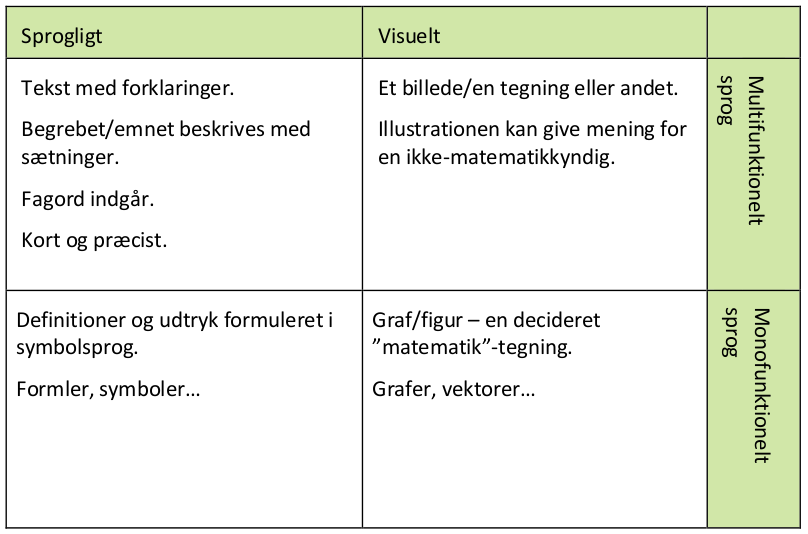
\includegraphics[width=.9\linewidth]{img/duval.png}
\end{center}

\begin{itemize}
\item Det er jeres opgave at udfylde de tomme felter.

\item Når I har besvaret alle tre opgaver, overvej med jer selv, hvilke overgange, som er "lette" og hvilke, som er "svære".
\end{itemize}

\newpage

\subsection*{Duvalopgave 1}
\label{sec:orgd152237}

Udfyld de tomme felter. I må gerne skrive mellemregninger og forklaringer ved siden af. Felterne er mest tænkt til at indikere, hvilke af Duvals fire rum, som er udfyldt og hvilke I skal oversætte til.

\begin{center}
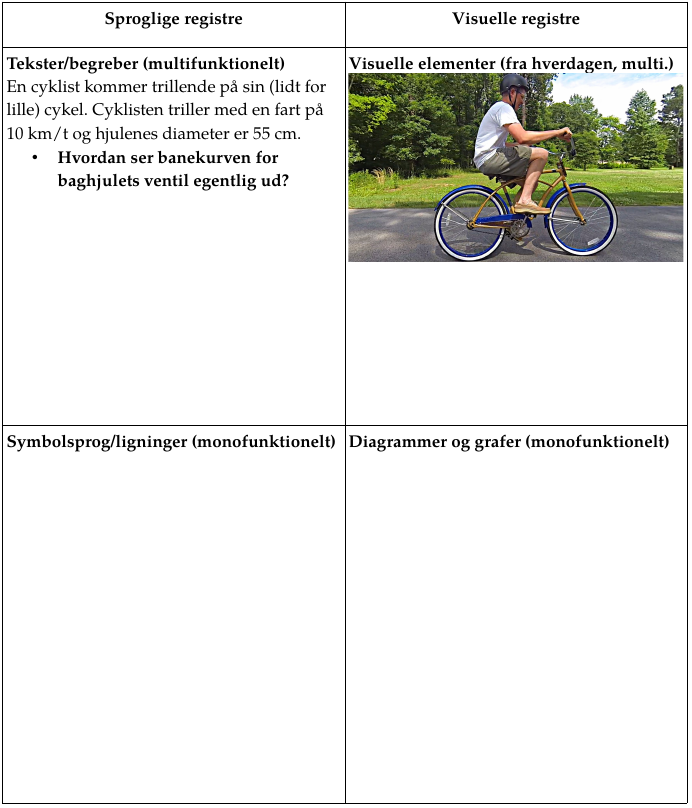
\includegraphics[width=.9\linewidth]{img/duvalopgave_1.png}
\end{center}


\newpage

\subsection*{Duvalopgave 2}
\label{sec:orgb07fc2a}

Udfyld de tomme felter. I må gerne skrive mellemregninger og forklaringer ved siden af. Felterne er mest tænkt til at indikere, hvilke af Duvals fire rum, som er udfyldt og hvilke I skal oversætte til.

\begin{center}
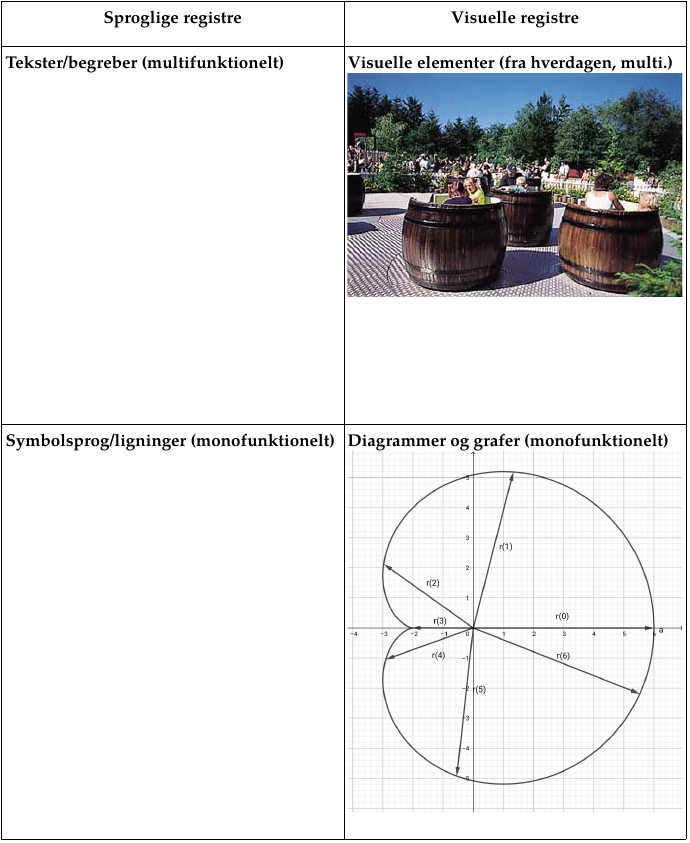
\includegraphics[width=.9\linewidth]{img/duvalopgave_2.png}
\end{center}


\subsection*{Duvalopgave 3}
\label{sec:org70073d4}

Udfyld de tomme felter. I må gerne skrive mellemregninger og forklaringer ved siden af. Felterne er mest tænkt til at indikere, hvilke af Duvals fire rum, som er udfyldt og hvilke I skal oversætte til.

\begin{center}
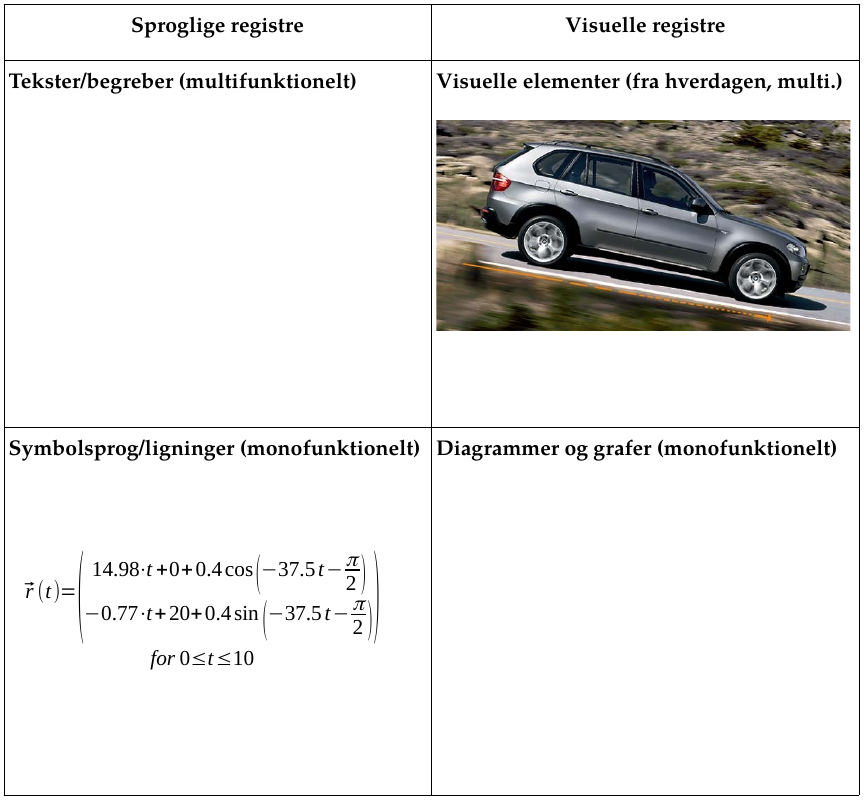
\includegraphics[width=.9\linewidth]{img/duvalopgave_3.png}
\end{center}

\newpage

\section*{Formelsamling til vektorfunktioner}
\label{sec:org555e88d}

Jeres sidste opgave er, at skrive jeres egen formelsamling til vektorfunktioner.

I kan formelsamlingen fra matematikbogen her: \url{https://mathtxa.systime.dk/?id=p386}, og lade jer inspirere af den.

Det vigtigste er dog, \textbf{at I selv skriver det hele ind. Formlerne skal skrives i en formeleditor og teksten skal I også selv skrive. Ikke noget med at copy-paste eller tager screenshots.}

Pointen med denne opgave er, at I får set alle formlerne og får bearbejdet dem ved selv at skrive dem ind.
\end{document}